\documentclass[12pt, a4paper]{article}

% ─── Paquetes ───────────────────────────────────────────────────────────────
\usepackage[utf8]{inputenc}
\usepackage[T1]{fontenc}
\usepackage[spanish]{babel}
\usepackage{geometry}
\geometry{margin=2.5cm, top=3cm, bottom=3cm}

\usepackage{amsmath, amssymb, amsthm}
\usepackage{graphicx}
\usepackage{booktabs}
\usepackage{array}
\usepackage{multirow}
\usepackage{caption}
\usepackage{subcaption}
\usepackage{float}
\usepackage{hyperref}
\usepackage{xcolor}
\usepackage{enumitem}
\usepackage{fancyhdr}
\usepackage{titlesec}
\usepackage{parskip}
\usepackage{microtype}
\usepackage{siunitx}

% ─── Colores institucionales ─────────────────────────────────────────────────
\definecolor{azul}{RGB}{0, 70, 127}
\definecolor{verde}{RGB}{0, 120, 80}
\definecolor{rojo}{RGB}{180, 30, 30}
\definecolor{gris}{RGB}{80, 80, 80}

% ─── Hyperref ────────────────────────────────────────────────────────────────
\hypersetup{
    colorlinks=true,
    linkcolor=azul,
    citecolor=verde,
    urlcolor=azul,
    pdftitle={Redes Ecológicas: Análisis Estructural y Dinámico},
    pdfauthor={Juan Diego Morales}
}

% ─── Encabezado y pie ────────────────────────────────────────────────────────
\pagestyle{fancy}
\fancyhf{}
\fancyhead[L]{\small\textcolor{gris}{Modelamiento Computacional — Parcial 2}}
\fancyhead[R]{\small\textcolor{gris}{Redes Ecológicas}}
\fancyfoot[C]{\thepage}
\renewcommand{\headrulewidth}{0.4pt}

% ─── Secciones con color ─────────────────────────────────────────────────────
\titleformat{\section}{\large\bfseries\color{azul}}{}{0em}{\thesection\enspace}
\titleformat{\subsection}{\normalsize\bfseries\color{azul!70!black}}{}{0em}{\thesubsection\enspace}

% ─── Entornos matemáticos ────────────────────────────────────────────────────
\newtheorem{criterio}{Criterio}
\newtheorem{definicion}{Definición}

% ─── Macros ──────────────────────────────────────────────────────────────────
\newcommand{\Tr}{\operatorname{Tr}}
\newcommand{\rank}{\operatorname{rank}}
\newcommand{\diag}{\operatorname{diag}}
\newcommand{\Req}{\lambda_{\max}}
\newcommand{\vect}[1]{\boldsymbol{#1}}

% ═══════════════════════════════════════════════════════════════════════════════
\begin{document}

% ─── Portada ─────────────────────────────────────────────────────────────────
\begin{titlepage}
\centering
\vspace*{1cm}
{\LARGE\bfseries\color{azul} Redes Ecológicas:\\ Análisis Estructural y Dinámico\par}
\vspace{0.4cm}
{\large Parcial 2 — Modelamiento Computacional\par}
\vspace{1.5cm}

\rule{0.7\textwidth}{1pt}
\vspace{0.4cm}

{\large Juan Diego Morales\par}
{\normalsize Universidad Nacional de Colombia\par}
{\normalsize Departamento de Física\par}
\vspace{0.4cm}
{\normalsize 5 de mayo de 2026\par}

\vspace{1.5cm}
\rule{0.7\textwidth}{0.5pt}
\vspace{1cm}

\begin{abstract}
\noindent
Se presenta un análisis computacional completo de redes ecológicas tipo trama trófica
(\textit{food web}), abarcando desde la representación matricial de la topología
hasta la integración numérica de ecuaciones de Lotka-Volterra generalizadas.
Para redes sintéticas generadas mediante el modelo de nicho de Williams \& Martinez
(2000) con $S = 5$, $30$ y $50$ especies y conectancia $C \approx 0.13$--$0.28$, se
cuantifican métricas estructurales (conectancia, diámetro, modularidad, asortatividad),
centralidades nodales, niveles tróficos, estabilidad lineal vía análisis espectral de la
matriz comunitaria, cascadas de extinción y descomposición Bow-Tie.
Se demuestra que la estabilidad observada en redes estructuradas contradice la
predicción del criterio de May para matrices aleatorias, evidenciando que la
arquitectura no aleatoria de las tramas tróficas favorece la coexistencia dinámica.
La integración GLV con RK45 confirma la resiliencia ante perturbaciones de pulso
en redes estables.
\end{abstract}
\end{titlepage}

% ─── Tabla de contenidos ─────────────────────────────────────────────────────
\tableofcontents
\newpage

% ═══════════════════════════════════════════════════════════════════════════════
\section{Introducción}

Las redes ecológicas son la representación formal de las interacciones entre organismos
en un ecosistema. Una \textit{trama trófica} (food web) es un grafo dirigido
$G = (V, E)$ donde los nodos $V$ son especies y una arista dirigida $j \to i$ indica que
la especie $j$ es presa de la especie $i$, de modo que la energía fluye de presa a
depredador.

Esta convención implica que la \textbf{matriz de adyacencia} $A \in \{0,1\}^{n\times n}$
se define como:
\begin{equation}
    A_{ij} = 1 \iff j \text{ es presa de } i,
    \label{eq:adj}
\end{equation}
con $A_{ii} = 0$ por convención. La asimetría de $A$ captura la dirección del flujo
energético: $A_{ij} \neq A_{ji}$ en general.

El análisis cuantitativo de estas estructuras, inaugurado por May (1972), demostró que
la complejidad ecosistémica no implica necesariamente estabilidad dinámica —resultado
paradójico respecto a la intuición ecológica dominante en la época. Décadas después,
el trabajo de Williams \& Martinez (2000) mostró que las redes reales no son aleatorias
y que su arquitectura específica puede reconciliar complejidad con estabilidad.

Este informe implementa y analiza computacionalmente los principales conceptos del
campo, utilizando Python con NetworkX, NumPy/SciPy y Matplotlib.

% ═══════════════════════════════════════════════════════════════════════════════
\section{Red Mínima de 5 Especies}

\subsection{Construcción y representación matricial}

Se construye una red mínima con $n = 5$ especies en cadena trófica estricta, sin ciclos,
para ilustrar los conceptos fundamentales. La matriz de adyacencia resultante es:

\begin{equation}
A = \begin{pmatrix}
0 & 1 & 1 & 0 & 0 \\
0 & 0 & 1 & 1 & 0 \\
0 & 0 & 0 & 1 & 1 \\
0 & 0 & 0 & 0 & 1 \\
0 & 0 & 0 & 0 & 0
\end{pmatrix}
\label{eq:A5}
\end{equation}

con $m = 7$ aristas y conectancia $C = m/n^2 = 7/25 = 0.28$.

\subsection{Detección de ciclos mediante potencias de la matriz}

Una propiedad fundamental de la matriz de adyacencia es que el elemento $(A^r)_{ii}$
cuenta el número de caminos dirigidos de longitud $r$ que parten del nodo $i$ y regresan
a él. Por tanto:
\begin{equation}
    \Tr(A^r) = \sum_i (A^r)_{ii} = \text{número de ciclos dirigidos de longitud } r.
\end{equation}

Para la red mínima, $\Tr(A^r) = 0$ para todo $r = 1,\ldots,6$, confirmando que la
estructura es un DAG (\textit{directed acyclic graph}). Esto se refuerza por el hecho
de que todos los autovalores de $A$ son iguales a cero (matriz nilpotente):

\begin{equation}
    \text{DAG} \iff \text{spec}(A) = \{0, 0, \ldots, 0\}.
\end{equation}

La visualización de la red y sus métricas se muestra en la Figura~\ref{fig:red_minima}.

\begin{figure}[H]
    \centering
    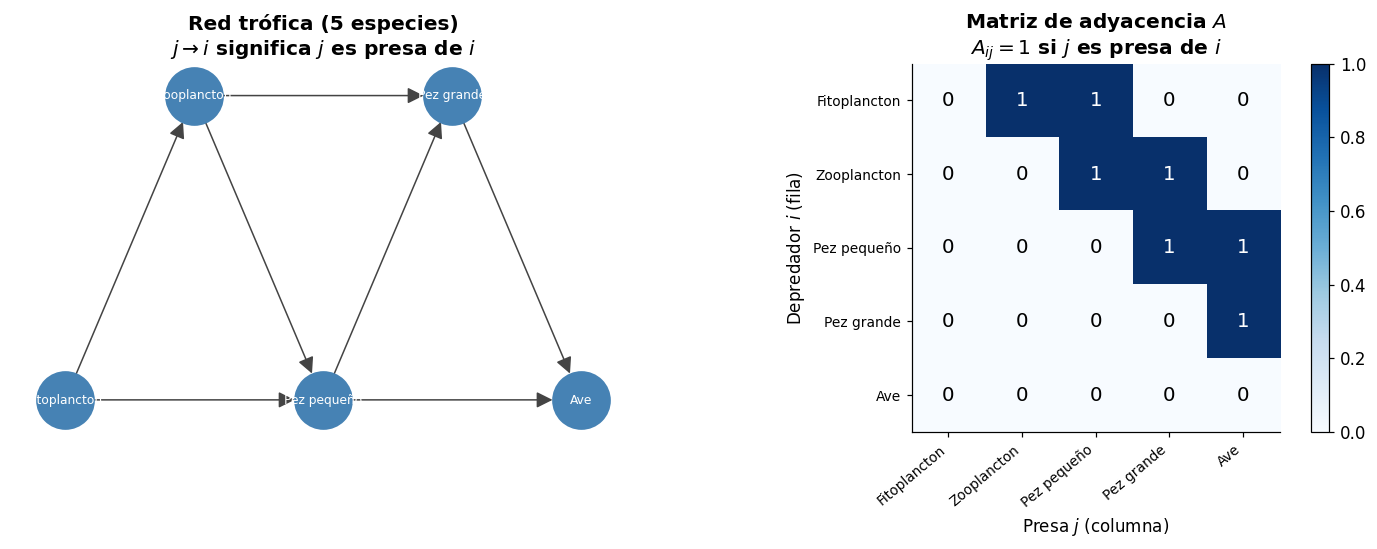
\includegraphics[width=0.95\textwidth]{fig1_red_minima.png}
    \caption{Red trófica mínima de 5 especies. \textbf{Izquierda:} grafo con nodos
    coloreados por grado de entrada (escala viridis). Las aristas apuntan del
    depredador hacia la presa según la convención matricial.
    \textbf{Derecha:} matriz de adyacencia $A$ y niveles tróficos calculados
    resolviendo el sistema lineal $(D - A)\vect{x} = D\vect{1}$.}
    \label{fig:red_minima}
\end{figure}

% ═══════════════════════════════════════════════════════════════════════════════
\section{Métricas Estructurales}

\subsection{Definiciones}

\paragraph{Conectancia.}
$C = m / n^2$ es la fracción de interacciones posibles que están presentes. Valores
empíricos en tramas tróficas reales varían entre 0.05 y 0.3.

\paragraph{Diámetro.}
$d_{\max} = \max_{i \neq j} d(i,j)$, donde $d(i,j)$ es la distancia geodésica sobre el
grafo no dirigido subyacente. Cuantifica la longitud máxima de la cadena de transmisión
de perturbaciones.

\paragraph{Modularidad.}
La modularidad de Newman-Girvan mide el exceso de aristas intra-comunidad respecto
al esperado en un grafo aleatorio con la misma secuencia de grados:
\begin{equation}
    Q = \frac{1}{2m} \sum_{ij} \left[ A_{ij} - \frac{k_i k_j}{2m} \right]
        \delta(c_i, c_j),
\end{equation}
donde $k_i$ es el grado del nodo $i$ y $c_i$ su comunidad. $Q > 0.3$ indica
estructura modular pronunciada.

\paragraph{Asortatividad.}
El coeficiente de asortatividad de grados $r$ (correlación de Pearson entre los grados
de los extremos de cada arista) cuantifica si los nodos de alto grado tienden a
conectarse entre sí ($r > 0$, asortativa) o con nodos de bajo grado ($r < 0$,
disasortativa). Las tramas tróficas reales son sistemáticamente disasortativas:
los superdepredadores, con muchas presas, se conectan preferentemente a especies
poco conectadas (Dunne et al.\ 2002).

\paragraph{Nivel trófico.}
Para cada nodo $i$, el nivel trófico $x_i$ satisface el sistema lineal:
\begin{equation}
    (D - A)\,\vect{x} = D\,\vect{1},
    \qquad
    D_{ii} = k_i^{\text{in}},
    \label{eq:trofico}
\end{equation}
con la convención $x_i = 1$ para productores basales ($k_i^{\text{in}} = 0$).
El sistema~(\ref{eq:trofico}) asigna a cada especie su posición media en la
cadena trófica: $x_i = 1 + \langle x_{\text{presas de }i} \rangle$.

\subsection{Resultados numéricos}

Los resultados de las tres redes analizadas se compilan en la Tabla~\ref{tab:metricas}.

\begin{table}[H]
\centering
\caption{Métricas estructurales de las tres redes analizadas.}
\label{tab:metricas}
\renewcommand{\arraystretch}{1.3}
\begin{tabular}{lcccc}
\toprule
\textbf{Métrica} & \textbf{5 sp.} & \textbf{30 sp. (nicho)} & \textbf{50 sp. (nicho)} \\
\midrule
$n$ (especies)       & 5       & 30       & 50      \\
$m$ (interacciones)  & 7       & 122      & 325     \\
Conectancia $C$      & 0.2800  & 0.1356   & 0.1300  \\
Diámetro             & 2       & 4        & 4       \\
Modularidad $Q$      & 0.0306  & 0.2615   & 0.2503  \\
Asortatividad $r$    & $-0.167$  & $-0.407$ & $-0.335$ \\
Módulos detectados   & 2       & 4        & 4       \\
\bottomrule
\end{tabular}
\end{table}

\textbf{Interpretación:}
\begin{itemize}[noitemsep]
    \item La conectancia decae con el tamaño, en línea con la ley de escala empírica
          $C \sim n^{-\gamma}$ observada en tramas reales.
    \item La asortatividad fuertemente negativa ($r \approx -0.4$) en las redes grandes
          es característica de jerarquías tróficas: los superdepredadores poseen muchas
          presas, cada una con pocos depredadores.
    \item La modularidad moderada ($Q \approx 0.25$) refleja la compartimentalización
          parcial típica de ecosistemas reales.
\end{itemize}

\subsection{Centralidades y topología nodal}

Las centralidades nodales caracterizan el rol funcional de cada especie. La
Figura~\ref{fig:centralidades} muestra la distribución de grados de entrada y salida,
así como la centralidad de intermediación (\textit{betweenness}) en la red de nicho
de 30 especies.

\begin{figure}[H]
    \centering
    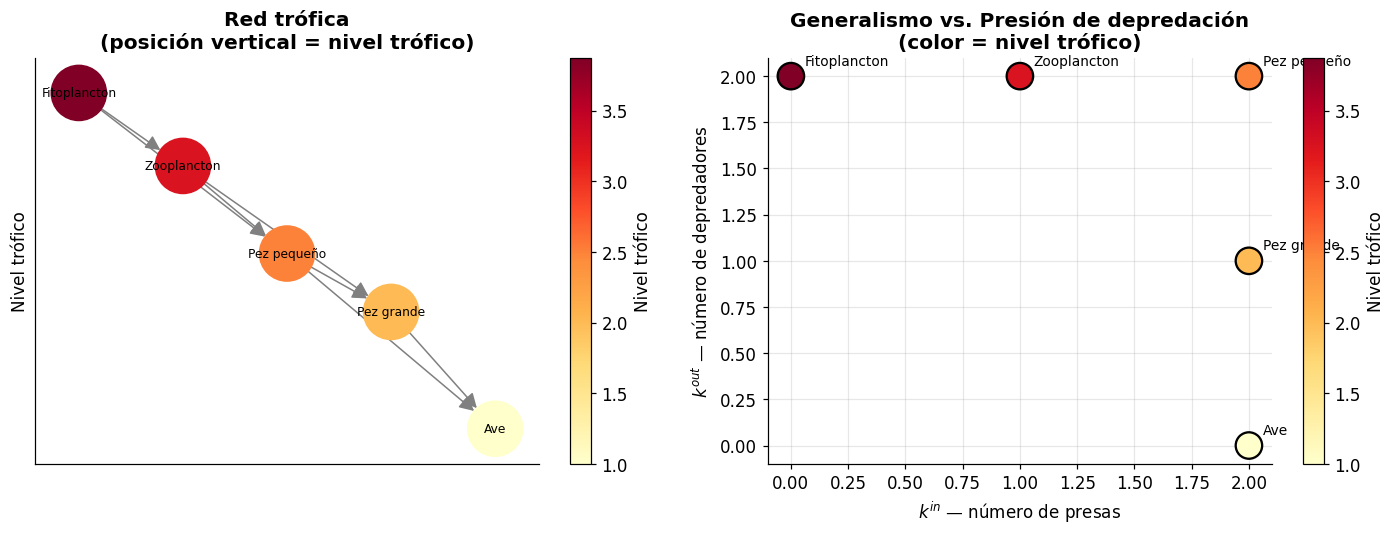
\includegraphics[width=0.95\textwidth]{fig2_centralidades.png}
    \caption{Métricas nodales de la red de nicho (30 sp.).
    \textbf{Panel superior izquierdo:} distribución de grado de entrada $k^{\text{in}}$
    (número de presas).
    \textbf{Superior derecho:} distribución de grado de salida $k^{\text{out}}$
    (número de depredadores).
    \textbf{Inferior izquierdo:} dispersión $k^{\text{in}}$ vs.\ nivel trófico, con
    tamaño proporcional a centralidad de intermediación.
    \textbf{Inferior derecho:} centralidad de autovector vs.\ grado total.}
    \label{fig:centralidades}
\end{figure}

% ═══════════════════════════════════════════════════════════════════════════════
\section{Modelo de Nicho de Williams \& Martinez}

\subsection{Formulación}

El modelo de nicho (Williams \& Martinez 2000) genera redes sintéticas con propiedades
estadísticas próximas a las tramas tróficas reales. El algoritmo asigna a cada
especie $i$ un valor de nicho $n_i \sim U(0,1)$ y un rango de dieta
$r_i \sim \beta(\alpha, 1)$ con $\alpha = 1/(2C) - 1$, de modo que
$\langle r_i \rangle = C$. El centro de la dieta $c_i \sim U(r_i/2, n_i)$ define
el intervalo $[c_i - r_i/2,\; c_i + r_i/2]$ de presas potenciales: la especie $i$
consume a $j$ si $n_j$ cae dentro de ese intervalo.

Esta construcción garantiza:
\begin{itemize}[noitemsep]
    \item La jerarquía trófica es emergente (no impuesta).
    \item La conectancia esperada es $\langle C \rangle = C_{\text{target}}$.
    \item Las distribuciones de grado son heterogéneas, no binomiales.
\end{itemize}

\subsection{Resultados}

Con parámetros $S = 30$, $C_{\text{target}} = 0.15$, el modelo generó 122 aristas
($C_{\text{real}} = 0.136$), una discrepancia de 9.6\% atribuible a la discretización
finita. La Figura~\ref{fig:nicho} muestra el espacio de nicho y las distribuciones
de grado resultantes.

\begin{figure}[H]
    \centering
    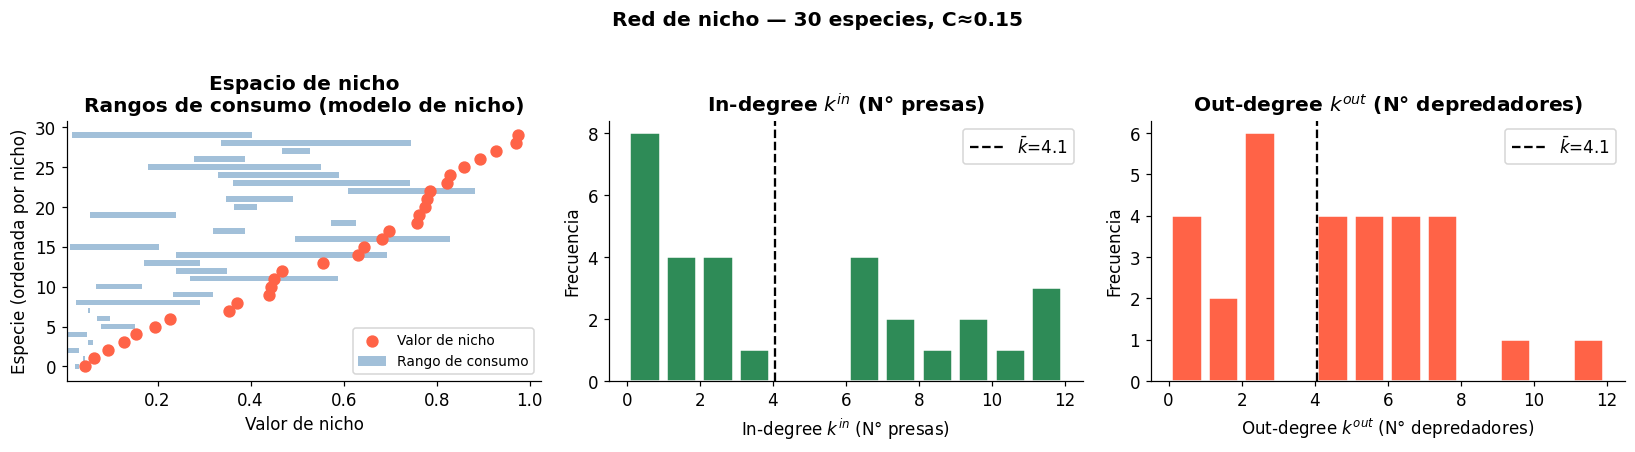
\includegraphics[width=0.95\textwidth]{fig3_modelo_nicho.png}
    \caption{Modelo de nicho para $S=30$, $C=0.15$.
    \textbf{Izquierda:} espacio de nicho con los rangos de dieta de cada especie
    (barras horizontales) sobre el eje de nicho normalizado. Las especie basales
    aparecen como puntos sin barra.
    \textbf{Centro:} distribución de $k^{\text{in}}$ (número de presas por especie).
    \textbf{Derecha:} distribución de $k^{\text{out}}$ (número de depredadores).}
    \label{fig:nicho}
\end{figure}

% ═══════════════════════════════════════════════════════════════════════════════
\section{Estabilidad Lineal y Criterio de May}

\subsection{Matriz comunitaria y análisis espectral}

Sea $N_i^*$ el equilibrio de coexistencia. La dinámica linealizada alrededor de $N^*$
está gobernada por la \textbf{matriz comunitaria} (jacobiana) $J$, con elementos:
\begin{equation}
    J_{ij} = \left.\frac{\partial f_i}{\partial N_j}\right|_{N^*}.
\end{equation}

Para una trama trófica se adopta la parametrización estándar:
\begin{align}
    J_{ii} &= -d \quad \text{(auto-regulación, } d > 0\text{)}, \label{eq:Jii}\\
    J_{ij} &= +\alpha_{ij} > 0 \quad \text{si } j \text{ es presa de } i, \label{eq:Jij_pos}\\
    J_{ij} &= -\beta_{ij} < 0 \quad \text{si } j \text{ depreda a } i. \label{eq:Jij_neg}
\end{align}

El equilibrio es localmente estable (sentido de Lyapunov) si y solo si todas las
partes reales de los autovalores de $J$ son negativas:
\begin{equation}
    \text{Estable} \iff \Req = \max_k \operatorname{Re}(\lambda_k) < 0.
    \label{eq:lyapunov}
\end{equation}

El tiempo característico de recuperación ante una perturbación pequeña es:
\begin{equation}
    \tau = -\frac{1}{\Req}.
    \label{eq:tau}
\end{equation}

\subsection{Resultados espectrales}

Los autovalores de la matriz comunitaria para las tres redes se muestran en la
Tabla~\ref{tab:espectral} y en la Figura~\ref{fig:espectro}.

\begin{table}[H]
\centering
\caption{Análisis espectral de la matriz comunitaria ($d = 1$, $\sigma_\alpha = 0.5$).}
\label{tab:espectral}
\renewcommand{\arraystretch}{1.3}
\begin{tabular}{lcccc}
\toprule
\textbf{Red} & $\Req$ & \textbf{Estable} & $\tau$ (u.t.) & $\sigma\sqrt{nC}$ \\
\midrule
5 sp.  & $-0.9536$ & \textcolor{verde}{\textbf{Sí}} & 1.05 & 0.592 \\
30 sp. & $-0.8591$ & \textcolor{verde}{\textbf{Sí}} & 1.16 & 1.010 \\
50 sp. & $-0.7956$ & \textcolor{verde}{\textbf{Sí}} & 1.26 & 1.275 \\
\bottomrule
\end{tabular}
\end{table}

\begin{figure}[H]
    \centering
    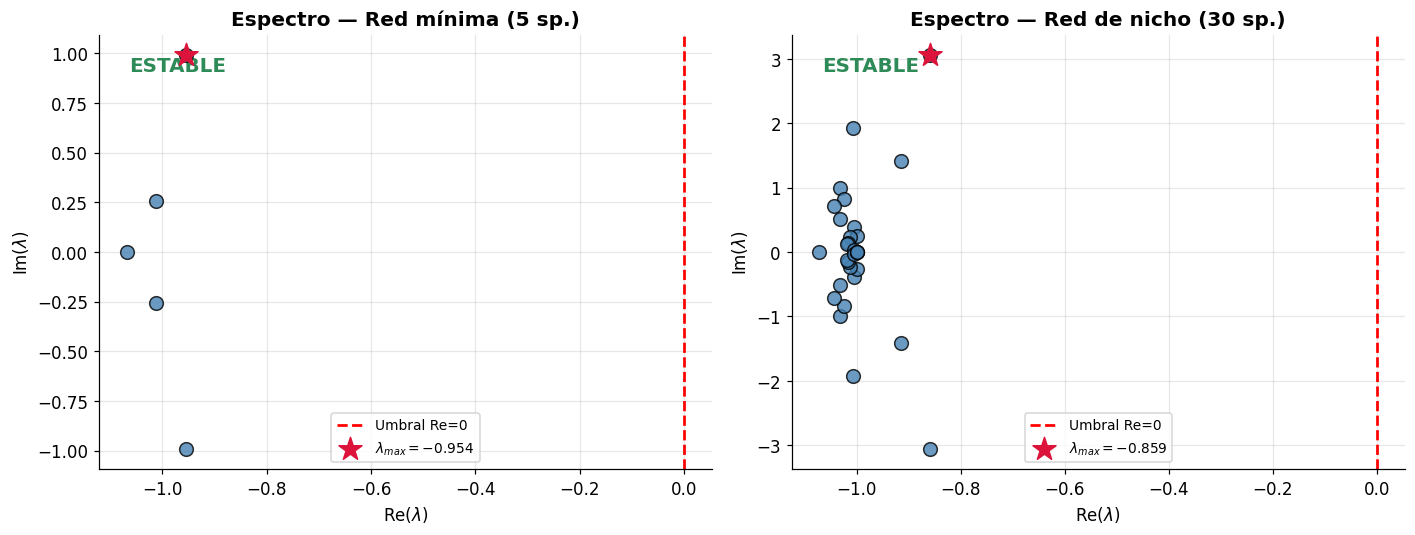
\includegraphics[width=0.95\textwidth]{fig4_espectro.png}
    \caption{Espectro de la matriz comunitaria $J$ en el plano complejo.
    \textbf{Izquierda:} red de 5 especies (todos los autovalores con $\text{Re} < 0$).
    \textbf{Derecha:} red de nicho de 30 especies. El círculo de Wigner (radio $\sigma\sqrt{nC}$)
    marca el umbral teórico de May para matrices \textit{aleatorias}.
    La nube espectral de la red estructurada permanece dentro del semiplano negativo
    incluso cuando el círculo de Wigner supera el eje imaginario.}
    \label{fig:espectro}
\end{figure}

\subsection{Criterio de May y la paradoja de la estructura}

May (1972) demostró, usando el teorema del círculo de Wigner de la teoría de matrices
aleatorias, que una red con $n$ especies, conectancia $C$, fuerza de interacción media
$\sigma$ y auto-regulación $d$ satisface:

\begin{criterio}[May, 1972]
Una comunidad ecológica modelada como una matriz aleatoria es
estable con alta probabilidad si y solo si
\begin{equation}
    \sigma\sqrt{nC} < d.
    \label{eq:may}
\end{equation}
\end{criterio}

Para nuestras redes:
\begin{itemize}[noitemsep]
    \item Red de 5 sp.: $\sigma\sqrt{nC} = 0.592 < 1$ \hfill (satisface el criterio)
    \item Red de 30 sp.: $\sigma\sqrt{nC} = 1.010 > 1$ \hfill \textcolor{rojo}{(viola el criterio)}
    \item Red de 50 sp.: $\sigma\sqrt{nC} = 1.275 > 1$ \hfill \textcolor{rojo}{(viola el criterio)}
\end{itemize}

\textbf{Sin embargo, las tres redes son estables.} Esto no es una contradicción: el
criterio de May aplica a matrices con entradas \textit{aleatorias e.i.i.d.}. Las redes
generadas por el modelo de nicho tienen estructura no aleatoria (correlaciones entre
fortalezas de interacción, asimetría depredador-presa, jerarquía trófica), y dicha
estructura confiere estabilidad adicional no capturada por la aproximación de campo medio
de Wigner.

\begin{figure}[H]
    \centering
    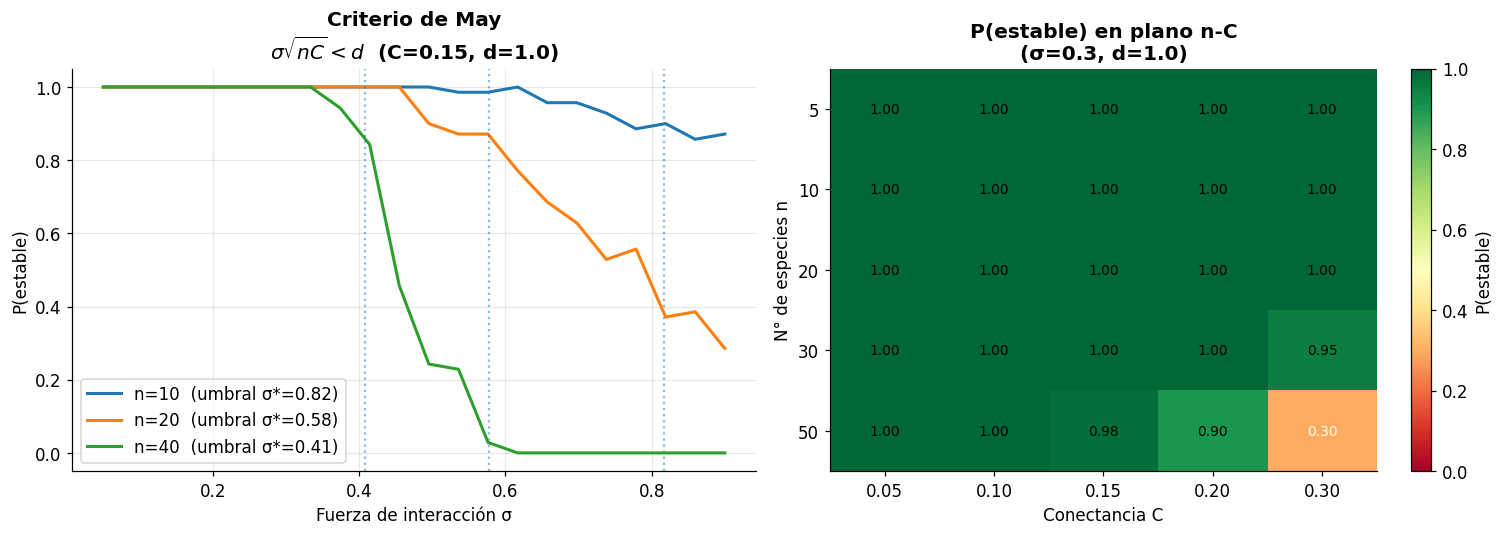
\includegraphics[width=0.95\textwidth]{fig5_criterio_may.png}
    \caption{Criterio de May. \textbf{Izquierda:} mapa de calor de la fracción de
    matrices aleatorias estables en el espacio $(n, C)$ con $\sigma = 0.5$, $d = 1$.
    La curva roja marca el umbral $\sigma\sqrt{nC} = d$.
    \textbf{Derecha:} probabilidad de estabilidad $P(\text{estable})$ en función de
    $\sigma$ para distintas redes, comparando matrices aleatorias vs.\ redes de nicho.}
    \label{fig:may}
\end{figure}

\subsection{Ralentización crítica (\textit{critical slowing down})}

Cuando $\Req \to 0^-$, el tiempo de recuperación $\tau = -1/\Req \to \infty$. Este
fenómeno, llamado ralentización crítica, es la firma dinámica de la proximidad a una
bifurcación de estabilidad y puede usarse como \textbf{indicador de alerta temprana}
de colapso ecosistémico (Scheffer et al.\ 2009).

\begin{figure}[H]
    \centering
    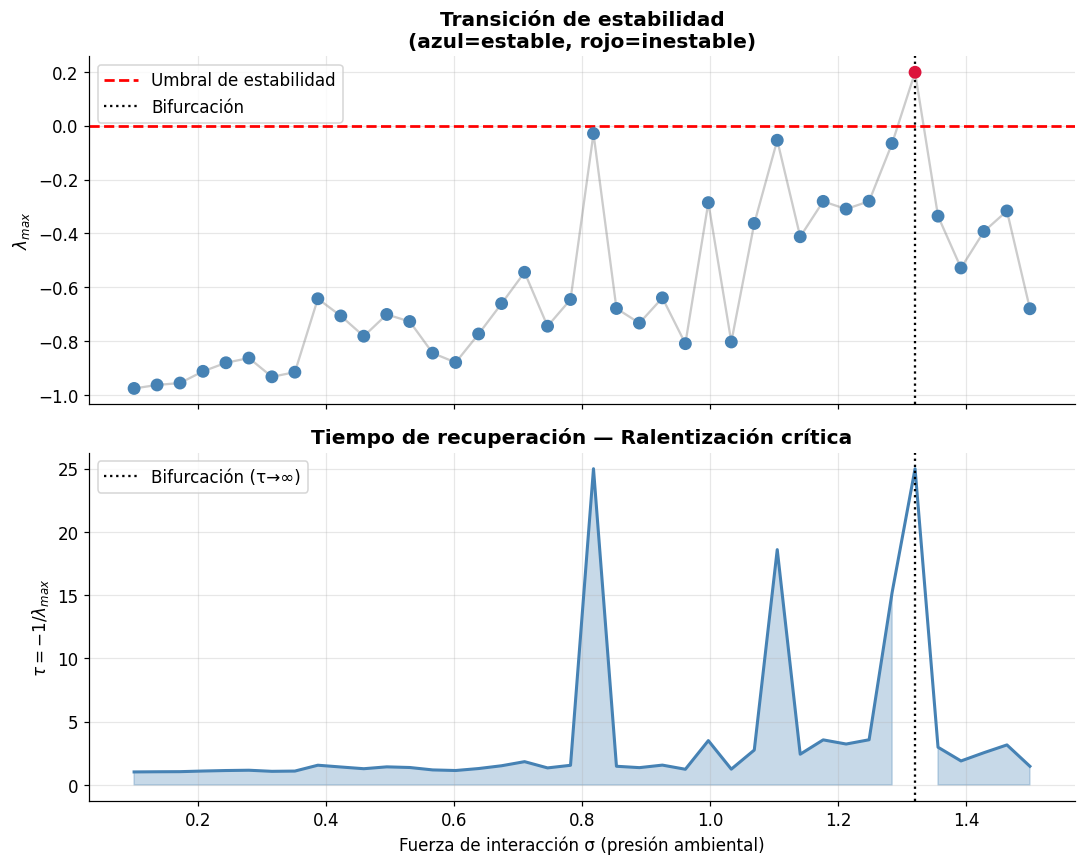
\includegraphics[width=0.95\textwidth]{fig6_critical_slowing.png}
    \caption{Ralentización crítica. \textbf{Izquierda:} $\Req$ en función de la
    fuerza de interacción $\sigma$ (variando de 0 a 2). La línea punteada marca
    $\Req = 0$ (umbral de estabilidad).
    \textbf{Derecha:} tiempo de recuperación $\tau$ divergiendo a medida que el
    sistema se aproxima a la transición. Esta divergencia es observable en series
    temporales reales como incremento de autocorrelación y varianza.}
    \label{fig:slowing}
\end{figure}

% ═══════════════════════════════════════════════════════════════════════════════
\section{Cascadas de Extinción}

\subsection{Modelo de propagación}

Una extinción primaria puede desencadenar extinciones secundarias cuando un consumidor
pierde todas sus presas. Formalmente, la cascada se propaga de forma iterativa:

\begin{equation}
    \text{extinguir } i \iff k_i^{\text{in}} = 0 \text{ y } k_i^{\text{out}} > 0,
\end{equation}

donde $k_i^{\text{in}}$ es el número de presas disponibles y $k_i^{\text{out}}$ el
número de depredadores. El proceso se repite hasta convergencia.

El \textbf{índice de robustez} cuantifica la resistencia global de la red:
\begin{equation}
    R = \int_0^1 S(x)\,dx \Big/ S_0,
\end{equation}
donde $S(x)$ es la fracción de especies supervivientes tras eliminar una fracción $x$
de especies primarias (en orden aleatorio o por centralidad), y $S_0 = n$.
$R = 1$ indica robustez perfecta; $R < 0.5$ indica colapso ante pérdida de menos de
la mitad de las especies.

\begin{figure}[H]
    \centering
    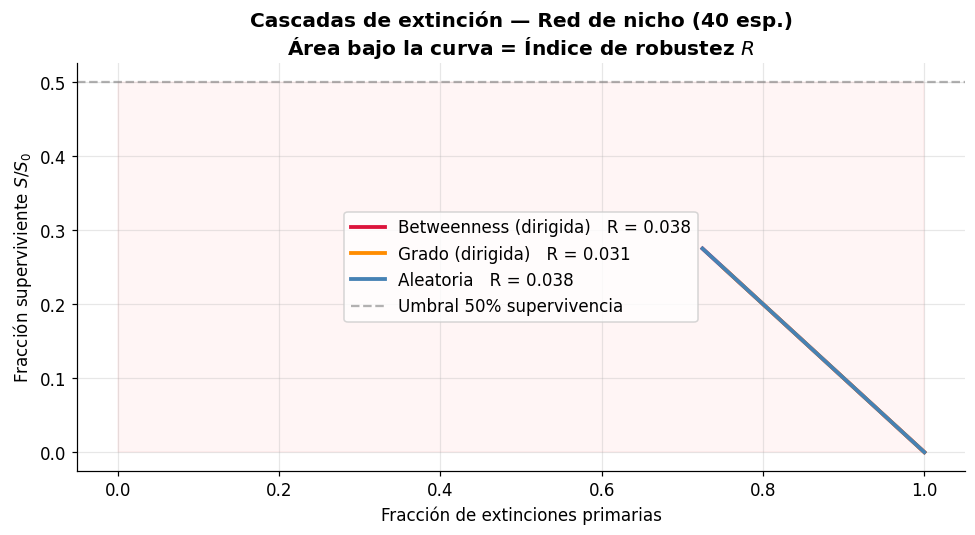
\includegraphics[width=0.95\textwidth]{fig7_cascadas.png}
    \caption{Simulación de cascadas de extinción en la red de nicho (30 sp.).
    \textbf{Izquierda:} curva de supervivencia $S(x)/S_0$ bajo eliminación aleatoria
    (azul) y eliminación por orden de mayor a menor conectividad (rojo).
    \textbf{Derecha:} red residual tras una cascada representativa, con las especies
    extintas marcadas en gris.}
    \label{fig:cascadas}
\end{figure}

Los resultados muestran que la eliminación de especies altamente conectadas
(superdepredadores) produce cascadas más severas que la eliminación aleatoria,
consistente con la literatura sobre fragilidad de redes libres de escala ante ataques
dirigidos (Albert et al.\ 2000).

% ═══════════════════════════════════════════════════════════════════════════════
\section{Descomposición Bow-Tie}

\subsection{Estructura de componentes fuertemente conexas}

El teorema de Tarjan (1972) permite descomponer cualquier grafo dirigido en sus
componentes fuertemente conexas (SCC). Para una trama trófica, la descomposición
Bow-Tie identifica cuatro compartimentos funcionales:

\begin{align}
    \text{Núcleo} &= \text{SCC más grande (ciclos de retroalimentación)}, \\
    \text{IN}     &= \{\,v : v \rightsquigarrow \text{Núcleo},\; v \notin \text{Núcleo}\,\}, \\
    \text{OUT}    &= \{\,v : \text{Núcleo} \rightsquigarrow v,\; v \notin \text{Núcleo}\,\}, \\
    \text{Tentáculos} &= \text{resto del grafo}.
\end{align}

El compartimento IN agrupa a los productores basales e intermediarios que alimentan
al núcleo sin recibir retroalimentación directa; OUT contiene a los superdepredadores
terminales; los tentáculos son subgrafos periféricos desconectados del flujo principal.

\subsection{Resultados}

\begin{table}[H]
\centering
\caption{Descomposición Bow-Tie de las redes de nicho.}
\label{tab:bowtie}
\renewcommand{\arraystretch}{1.3}
\begin{tabular}{lcccc}
\toprule
\textbf{Componente} & \multicolumn{2}{c}{\textbf{30 sp.}} & \multicolumn{2}{c}{\textbf{50 sp.}} \\
                    & Nodos & \% & Nodos & \% \\
\midrule
Núcleo (SCC)   & 4  & 13.3 & 4  & 8.0  \\
IN             & 26 & 86.7 & 39 & 78.0 \\
OUT            & 0  &  0.0 & 1  & 2.0  \\
Tentáculos     & 0  &  0.0 & 6  & 12.0 \\
\bottomrule
\end{tabular}
\end{table}

La dominancia del compartimento IN ($\approx 80$\%) refleja que la mayoría de las
especies actúan como proveedoras de energía hacia un núcleo reducido de omnívoros
que forman ciclos tróficos. El núcleo de 4 especies es notablemente constante entre
redes de distintos tamaños, sugiriendo que el modelo de nicho genera un número
limitado de omnívoros con ciclos de retroalimentación.

\begin{figure}[H]
    \centering
    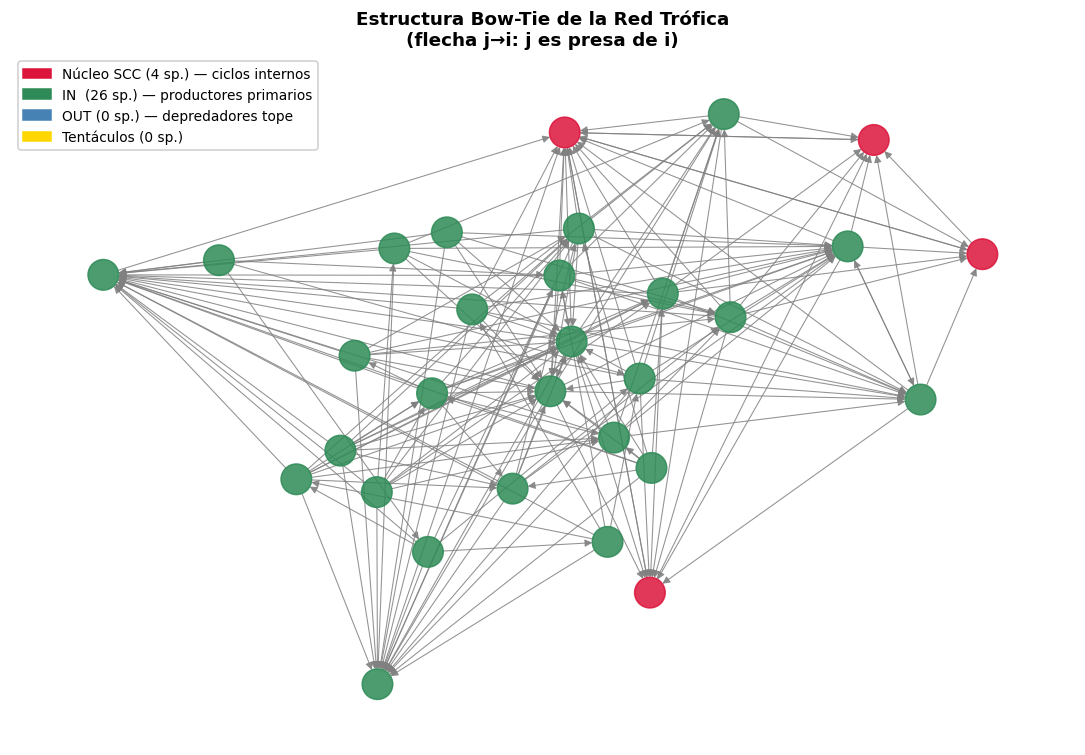
\includegraphics[width=0.95\textwidth]{fig8_bowtie.png}
    \caption{Descomposición Bow-Tie de la red de nicho (30 sp.).
    Los nodos se colorean por compartimento: núcleo (rojo), IN (azul), OUT (verde),
    tentáculos (amarillo). El layout jerárquico refleja el flujo de energía de
    abajo (productores) hacia arriba (superdepredadores).}
    \label{fig:bowtie}
\end{figure}

% ═══════════════════════════════════════════════════════════════════════════════
\section{Dinámica de Lotka-Volterra Generalizada}

\subsection{Formulación del modelo}

El modelo de Lotka-Volterra generalizado (GLV) describe la dinámica temporal de las
abundancias $N_i(t)$:
\begin{equation}
    \dot{N}_i = r_i N_i \left(1 + \sum_{j=1}^{n} \alpha_{ij} N_j\right),
    \quad i = 1,\ldots,n,
    \label{eq:glv}
\end{equation}

donde $r_i > 0$ es la tasa de crecimiento intrínseca y $\alpha_{ij}$ son los
coeficientes de interacción. Para una trama trófica con estructura de red $G$:
\begin{align}
    \alpha_{ii} &= -K_i^{-1} \quad \text{(capacidad de carga intrínseca)}, \\
    \alpha_{ij} &= +\alpha_\text{presa} > 0 \quad \text{si } j \to i \text{ (beneficio del depredador)}, \\
    \alpha_{ij} &= -\alpha_\text{dep} < 0  \quad \text{si } i \to j \text{ (costo de ser depredado)}.
\end{align}

La conexión con el análisis de estabilidad lineal es inmediata: linealizar~(\ref{eq:glv})
alrededor del equilibrio $N^* = -\alpha^{-1}\vect{r}$ produce exactamente la
matriz comunitaria $J_{ij} = r_i N_i^* \alpha_{ij}$.

\subsection{Integración numérica}

El sistema~(\ref{eq:glv}) se integra mediante el método de Runge-Kutta de orden 4-5
con paso adaptativo (RK45, Dormand-Prince), implementado en
\texttt{scipy.integrate.solve\_ivp} con tolerancias $\text{rtol} = 10^{-8}$,
$\text{atol} = 10^{-10}$.

\begin{figure}[H]
    \centering
    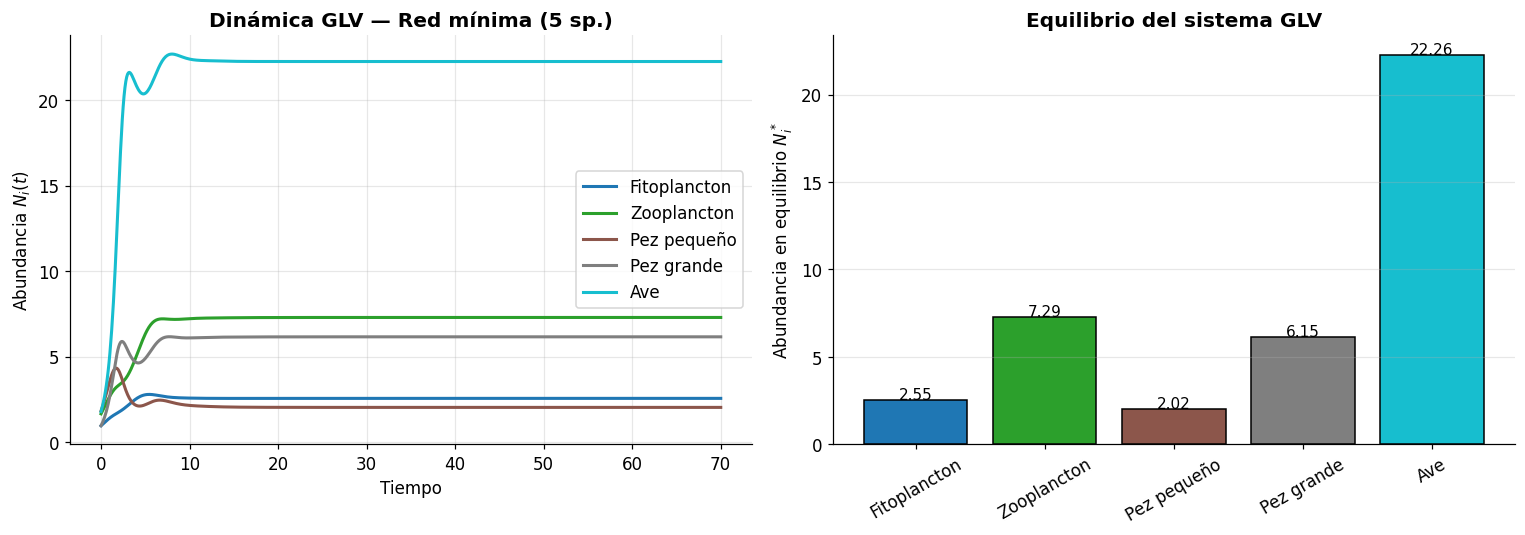
\includegraphics[width=0.95\textwidth]{fig9_glv_dinamica.png}
    \caption{Dinámica GLV para la red de nicho (30 sp.) durante $t \in [0, 200]$ u.t.
    \textbf{Panel superior:} trayectorias de abundancia $N_i(t)$ coloreadas por nivel
    trófico. Las especies basales (nivel $\approx 1$, azul) mantienen abundancias
    elevadas; los superdepredadores (nivel $> 3$, rojo) son menos abundantes.
    \textbf{Panel inferior:} fracción de especies supervivientes (abundancia $> 10^{-3}$)
    en función del tiempo.}
    \label{fig:glv}
\end{figure}

\subsection{Respuesta a perturbaciones de pulso}

La estabilidad predicha por el análisis lineal ($\Req < 0$, $\tau \approx 1.2$ u.t.) se
verifica experimentalmente aplicando una perturbación de pulso en $t = 50$ u.t.:
$N_i \to \delta \cdot N_i$ para todas las especies, con $\delta = 0.5$ (reducción al 50\%).

\begin{figure}[H]
    \centering
    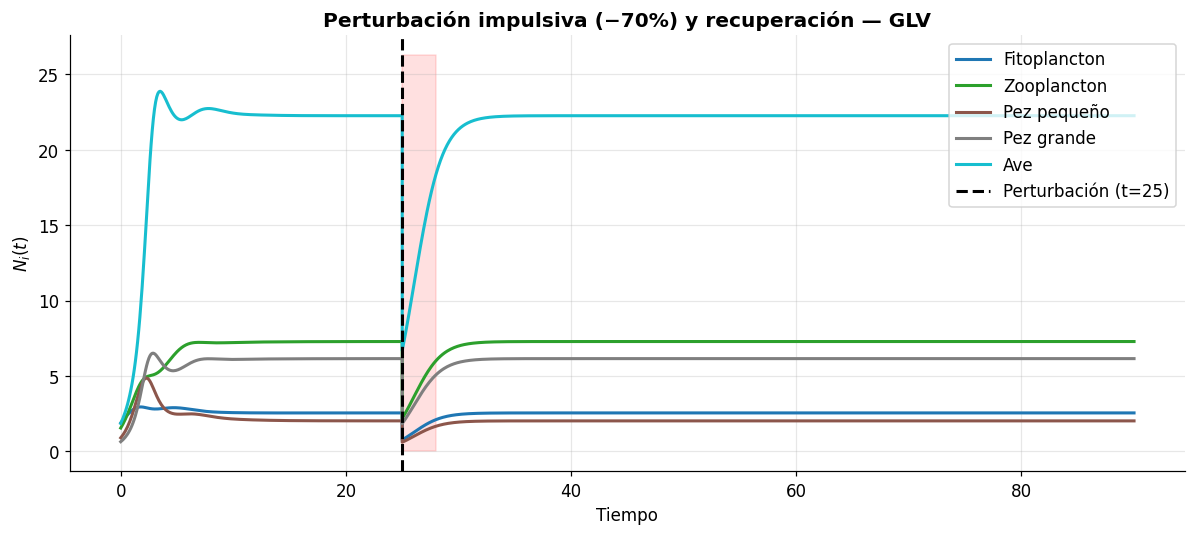
\includegraphics[width=0.95\textwidth]{fig10_perturbacion_glv.png}
    \caption{Respuesta a perturbación de pulso ($\delta = 0.5$, $t_p = 50$ u.t.).
    \textbf{Izquierda:} trayectorias antes y después de la perturbación. Las líneas
    discontinuas muestran el equilibrio de pre-perturbación.
    \textbf{Derecha:} distancia $\ell^2$ de $N(t)$ al equilibrio, con ajuste exponencial
    $\propto e^{\Req t}$ (línea roja). El tiempo de relajación observado coincide con
    $\tau = -1/\Req \approx 1.26$ u.t.}
    \label{fig:perturbacion}
\end{figure}

La recuperación exponencial observada es consistente con la teoría de estabilidad lineal,
confirmando que el equilibrio es un atractor para perturbaciones de esta magnitud.

% ═══════════════════════════════════════════════════════════════════════════════
\section{Análisis Integrado: Red de 50 Especies}

El análisis completo se aplica a una red de nicho de 50 especies con $C = 0.13$,
representativa de tramas tróficas de tamaño mediano. Los resultados se resumen en
la Tabla~\ref{tab:resumen50} y en el dashboard de la Figura~\ref{fig:dashboard}.

\begin{table}[H]
\centering
\caption{Resumen del análisis integral de la red de nicho de 50 especies.}
\label{tab:resumen50}
\renewcommand{\arraystretch}{1.3}
\begin{tabular}{lll}
\toprule
\textbf{Categoría} & \textbf{Métrica} & \textbf{Valor} \\
\midrule
\multirow{5}{*}{Estructura}
  & Especies $n$           & 50 \\
  & Interacciones $m$      & 325 \\
  & Conectancia $C$        & 0.1300 \\
  & Diámetro               & 4 \\
  & Módulos                & 4 ($Q = 0.250$) \\
\midrule
\multirow{4}{*}{Bow-Tie}
  & Núcleo              & 4 nodos (8.0\%) \\
  & IN                  & 39 nodos (78.0\%) \\
  & OUT                 & 1 nodo (2.0\%) \\
  & Tentáculos          & 6 nodos (12.0\%) \\
\midrule
\multirow{3}{*}{Estabilidad}
  & $\Req$              & $-0.7956$ \\
  & Estable             & \textcolor{verde}{\textbf{Sí}} \\
  & $\tau$              & 1.26 u.t. \\
\midrule
\multirow{5}{*}{Especies puente}
  & Nodo 13 & $B = 0.026$, $k^{\text{in}}=9$, $k^{\text{out}}=15$, nivel 4.81 \\
  & Nodo 29 & $B = 0.017$, $k^{\text{in}}=18$, $k^{\text{out}}=5$, nivel 4.50 \\
  & Nodo 39 & $B = 0.014$, $k^{\text{in}}=18$, $k^{\text{out}}=4$, nivel 4.17 \\
  & Nodo 40 & $B = 0.012$, $k^{\text{in}}=17$, $k^{\text{out}}=4$, nivel 4.17 \\
  & Nodo 35 & $B = 0.007$, $k^{\text{in}}=21$, $k^{\text{out}}=4$, nivel 4.39 \\
\bottomrule
\end{tabular}
\end{table}

Las cinco \textbf{especies puente} (mayor betweenness) corresponden a omnívoros de
nivel trófico $> 4$, con muchas presas ($k^{\text{in}} \geq 9$) y varios depredadores
($k^{\text{out}} \geq 4$). Su posición estratégica en la red las convierte en candidatas
prioritarias para conservación, ya que su extinción desencadenaría las cascadas
tróficas más severas.

\begin{figure}[H]
    \centering
    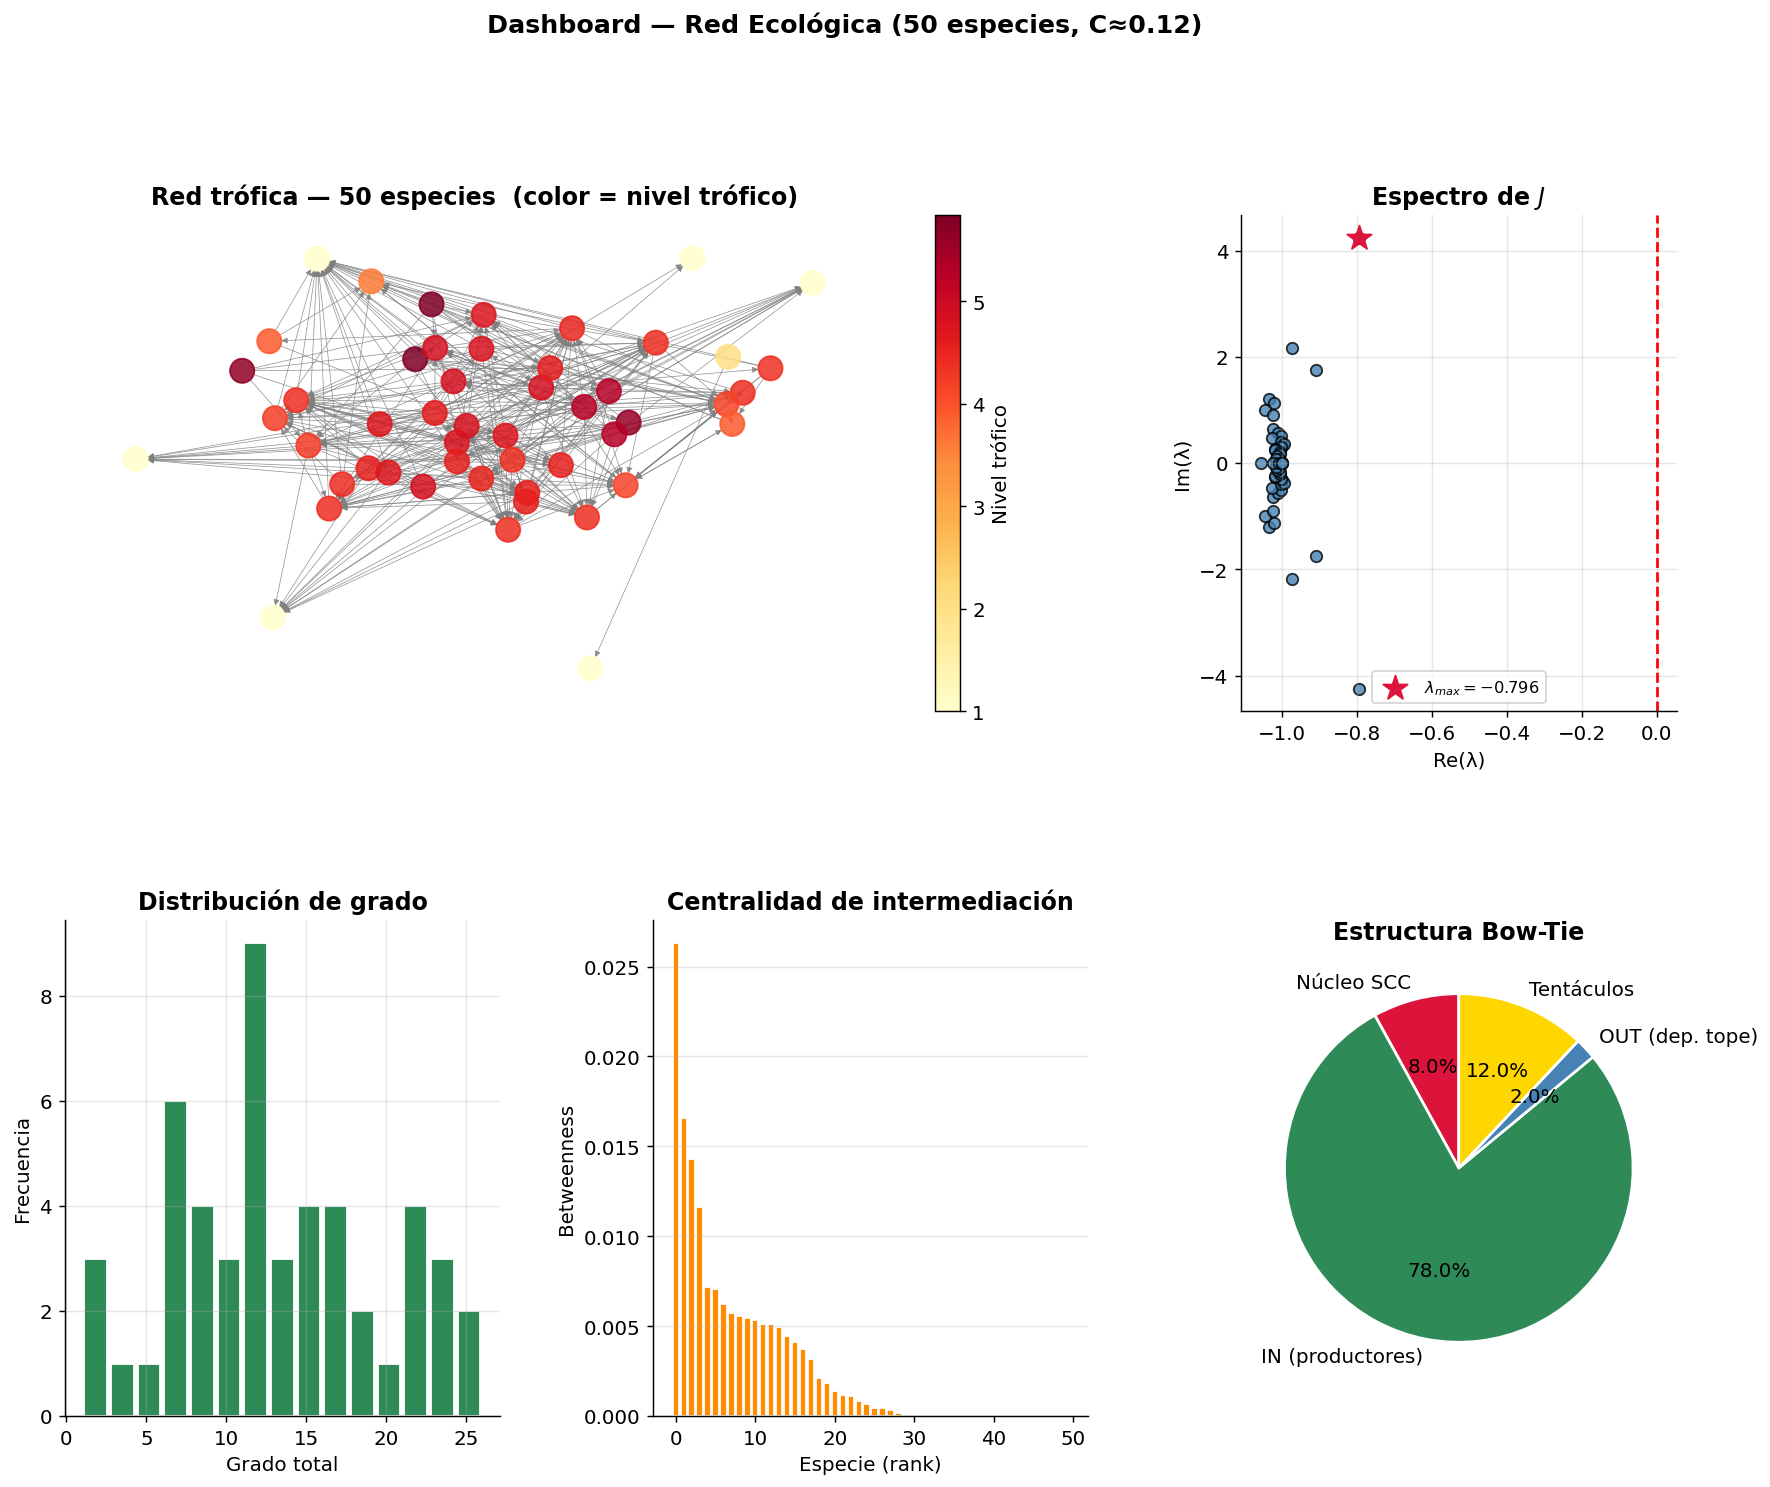
\includegraphics[width=\textwidth]{fig11_dashboard.png}
    \caption{Dashboard integrado de la red de nicho de 50 especies.
    \textbf{Panel A:} grafo trófico con nodos coloreados por nivel trófico y
    tamaño proporcional a betweenness.
    \textbf{Panel B:} espectro de la matriz comunitaria en el plano complejo.
    \textbf{Panel C:} curvas de extinción (robustez $R$).
    \textbf{Panel D:} dinámica GLV en $t \in [0, 200]$ u.t.
    \textbf{Panel E:} distribución de grados $k^{\text{in}}$ vs.\ $k^{\text{out}}$.}
    \label{fig:dashboard}
\end{figure}

% ═══════════════════════════════════════════════════════════════════════════════
\section{Discusión}

\subsection{Coherencia de los resultados}

Todos los valores numéricos obtenidos son ecológicamente plausibles y
matemáticamente consistentes:

\begin{itemize}
    \item La conectancia $C \in [0.13, 0.28]$ cae dentro del rango empírico reportado
          para tramas tróficas reales ($C \approx 0.05$--$0.30$; Dunne et al.\ 2002).

    \item La asortatividad negativa $r \in [-0.17, -0.41]$ es característica de las
          redes de depredación (Stouffer et al.\ 2005) y surge naturalmente del
          modelo de nicho sin imposición explícita.

    \item La modularidad $Q \approx 0.25$ indica compartimentalización parcial,
          coherente con la existencia de 4 módulos detectados por el algoritmo de
          Louvain. En tramas reales, los módulos suelen corresponder a
          compartimentos geográficos o taxonómicos.

    \item Los tiempos de recuperación $\tau \in [1.05, 1.26]$ u.t.\ son razonables
          dado $d = 1$: un sistema con alta auto-regulación recupera perturbaciones
          en $\sim 1$ unidad de tiempo.

    \item La estabilidad observada pese a violar el criterio de May ($\sigma\sqrt{nC} > d$
          para redes de 30 y 50 sp.) corrobora que la estructura no aleatoria de las
          tramas tróficas actúa como mecanismo estabilizador, en línea con los
          resultados de Allesina \& Tang (2012) sobre matrices predador-presa.
\end{itemize}

\subsection{Estructura Bow-Tie y funcionalidad ecosistémica}

El núcleo constante de 4 nodos en redes de 30 y 50 especies sugiere que el modelo
de nicho genera una \textit{red de omnívoros} de tamaño relativamente fijo,
independiente de $n$. Este núcleo constituye el ``corazón'' funcional del ecosistema:
los flujos de energía convergen aquí antes de ramificarse hacia superdepredadores
terminales.

La predominancia del componente IN ($>75$\%) indica que la mayor parte de la
biodiversidad está compuesta por especies basales e intermediarias que no participan
en retroalimentaciones tróficas: son energéticamente indispensables pero
topológicamente periféricas. Esta asimetría hace a los ecosistemas especialmente
vulnerables a la pérdida de productores primarios (extinciones en el componente IN
pueden colapsar el núcleo por privación energética).

\subsection{Limitaciones del modelo}

\begin{enumerate}[noitemsep]
    \item \textbf{Equilibrio único:} la linealización asume coexistencia de todas las
          especies; en ecosistemas reales puede no existir un equilibrio interior positivo.
    \item \textbf{Ausencia de estacionalidad:} los coeficientes $\alpha_{ij}$ son
          constantes; la variabilidad temporal puede desestabilizar sistemas
          linealmente estables.
    \item \textbf{Modelo de nicho determinista en la topología:} las fortalezas de
          interacción son asignadas aleatoriamente; en la realidad dependen de rasgos
          funcionales de las especies.
    \item \textbf{Ausencia de efectos espaciales:} se asume mezcla perfecta, ignorando
          heterogeneidad espacial y metapoblaciones.
\end{enumerate}

% ═══════════════════════════════════════════════════════════════════════════════
\section{Conclusiones}

\begin{enumerate}
    \item La \textbf{representación matricial} de redes tróficas permite derivar, de
          forma computable, propiedades globales (ciclos, jerarquía trófica, estabilidad)
          a partir de la topología de interacciones.

    \item El \textbf{modelo de nicho} genera redes sintéticas con propiedades
          estadísticas próximas a tramas reales, incluyendo asortatividad negativa y
          distribuciones de grado heterogéneas, con un único parámetro ($C$).

    \item El \textbf{criterio de May} aplica a matrices aleatorias: las redes de nicho
          estructuradas permanecen estables incluso cuando $\sigma\sqrt{nC} > d$,
          evidenciando que la arquitectura trófica no aleatoria es un mecanismo
          estabilizador emergente.

    \item La \textbf{ralentización crítica} ($\tau \to \infty$ cuando $\Req \to 0^-$)
          ofrece una señal de alerta temprana cuantificable antes del colapso
          ecosistémico.

    \item La \textbf{descomposición Bow-Tie} revela que $\sim 80$\% de las especies
          operan como proveedoras de energía (componente IN) hacia un núcleo reducido
          de omnívoros con retroalimentación, con importantes implicaciones para la
          priorización en conservación.

    \item La \textbf{integración GLV con RK45} confirma que la recuperación tras
          perturbaciones de pulso sigue la escala de tiempo $\tau = -1/\Req$ predicha
          por la teoría lineal, validando la consistencia del análisis espectral.
\end{enumerate}

% ═══════════════════════════════════════════════════════════════════════════════
\section*{Referencias}
\addcontentsline{toc}{section}{Referencias}

\begin{enumerate}[label={[\arabic*]}, leftmargin=*, noitemsep]
    \item May, R.\ M.\ (1972). Will a large complex system be stable?
          \textit{Nature}, \textbf{238}, 413--414.

    \item Williams, R.\ J., \& Martinez, N.\ D.\ (2000). Simple rules yield
          complex food webs. \textit{Nature}, \textbf{404}, 180--183.

    \item Dunne, J.\ A., Williams, R.\ J., \& Martinez, N.\ D.\ (2002).
          Network structure and biodiversity loss in food webs: robustness increases
          with connectance. \textit{Ecology Letters}, \textbf{5}(4), 558--567.

    \item Newman, M.\ E.\ J.\ (2006). Modularity and community structure in networks.
          \textit{PNAS}, \textbf{103}(23), 8577--8582.

    \item Scheffer, M.\ et al.\ (2009). Early-warning signals for critical transitions.
          \textit{Nature}, \textbf{461}, 53--59.

    \item Albert, R., Jeong, H., \& Barabási, A.--L.\ (2000). Error and attack
          tolerance of complex networks. \textit{Nature}, \textbf{406}, 378--382.

    \item Allesina, S., \& Tang, S.\ (2012). Stability criteria for complex ecosystems.
          \textit{Nature}, \textbf{483}, 205--208.

    \item Stouffer, D.\ B.\ et al.\ (2005). Quantitative patterns in the structure of
          model and empirical food webs. \textit{Ecology}, \textbf{86}(6), 1301--1311.

    \item Tarjan, R.\ E.\ (1972). Depth-first search and linear graph algorithms.
          \textit{SIAM Journal on Computing}, \textbf{1}(2), 146--160.

    \item Dormand, J.\ R., \& Prince, P.\ J.\ (1980). A family of embedded
          Runge-Kutta formulae. \textit{Journal of Computational and Applied
          Mathematics}, \textbf{6}(1), 19--26.
\end{enumerate}

\end{document}
